%% BioMed_Central_Tex_Template_v1.06
%%                                      %
%  bmc_article.tex            ver: 1.06 %
%                                       %

%%IMPORTANT: do not delete the first line of this template
%%It must be present to enable the BMC Submission system to
%%recognise this template!!

%%%%%%%%%%%%%%%%%%%%%%%%%%%%%%%%%%%%%%%%%
%%                                     %%
%%  LaTeX template for BioMed Central  %%
%%     journal article submissions     %%
%%                                     %%
%%          <8 June 2012>              %%
%%                                     %%
%%                                     %%
%%%%%%%%%%%%%%%%%%%%%%%%%%%%%%%%%%%%%%%%%


%%%%%%%%%%%%%%%%%%%%%%%%%%%%%%%%%%%%%%%%%%%%%%%%%%%%%%%%%%%%%%%%%%%%%
%%                                                                 %%
%% For instructions on how to fill out this Tex template           %%
%% document please refer to Readme.html and the instructions for   %%
%% authors page on the biomed central website                      %%
%% http://www.biomedcentral.com/info/authors/                      %%
%%                                                                 %%
%% Please do not use \input{...} to include other tex files.       %%
%% Submit your LaTeX manuscript as one .tex document.              %%
%%                                                                 %%
%% All additional figures and files should be attached             %%
%% separately and not embedded in the \TeX\ document itself.       %%
%%                                                                 %%
%% BioMed Central currently use the MikTex distribution of         %%
%% TeX for Windows) of TeX and LaTeX.  This is available from      %%
%% http://www.miktex.org                                           %%
%%                                                                 %%
%%%%%%%%%%%%%%%%%%%%%%%%%%%%%%%%%%%%%%%%%%%%%%%%%%%%%%%%%%%%%%%%%%%%%

%%% additional documentclass options:
%  [doublespacing]
%  [linenumbers]   - put the line numbers on margins

%%% loading packages, author definitions

%\documentclass[twocolumn]{bmcart}% uncomment this for twocolumn layout and comment line below
\documentclass{bmcart}

%%% Load packages
%\usepackage{amsthm,amsmath}
%\RequirePackage{natbib}
%\RequirePackage[authoryear]{natbib}% uncomment this for author-year bibliography
%\RequirePackage{hyperref}
\usepackage[utf8]{inputenc} %unicode support
%\usepackage[applemac]{inputenc} %applemac support if unicode package fails
%\usepackage[latin1]{inputenc} %UNIX support if unicode package fails
\usepackage{graphicx}

%% These have been added at the request of the MIT Libraries, because
%% some PDF conversions mess up the ligatures.  -LB, 1/22/2014
\usepackage{cmap}
\usepackage[T1]{fontenc}
\pagestyle{plain}

\usepackage{graphicx}
\usepackage[utf8]{inputenc}
\usepackage[T1]{fontenc} 
%\usepackage[latin1]{inputenc}
\usepackage{pifont} 
\usepackage{import}
\usepackage{amsmath}
\usepackage{multirow}
\usepackage{graphicx,url}
\usepackage{placeins}
\usepackage{adjustbox}
\usepackage[english]{babel}
\usepackage{lipsum}
\usepackage{multicol}
\usepackage{textcomp}
\usepackage{listings}
\usepackage{caption}
\usepackage{amsmath}
\usepackage{calc} 
\usepackage{array,url,kantlipsum}
\usepackage{algorithm}
\usepackage{algpseudocode}
\usepackage{lscape}
\usepackage{array}
\usepackage{natbib}
\usepackage{longtable}
\usepackage{booktabs}
\usepackage{txfonts}
\usepackage{colortbl}%
  \newcommand{\myrowcolour}{\rowcolor[gray]{0.925}}
\newenvironment{Figure}
  {\par\medskip\noindent\minipage{\linewidth}}
  {\endminipage\par\medskip}
  
\lstset{
language=Java,
basicstyle=\small\ttfamily,
numbers=left,
numbersep=5pt,
xleftmargin=20pt,
frame=tb,
framexleftmargin=20pt
}

\renewcommand*\thelstnumber{\arabic{lstnumber}:}

\DeclareCaptionFormat{mylst}{\hrule#1#2#3}
\captionsetup[lstlisting]{format=mylst,labelfont=bf,singlelinecheck=off,labelsep=space,font={normalsize,tt}}

\usepackage[framemethod=tikz]{mdframed}
\usepackage{lipsum}

\extrafloats{100}

%%%%%%%%%%%%%%%%%%%%%%%%%%%%%%%%%%%%%%%%%%%%%%%%%
%%                                             %%
%%  If you wish to display your graphics for   %%
%%  your own use using includegraphic or       %%
%%  includegraphics, then comment out the      %%
%%  following two lines of code.               %%
%%  NB: These line *must* be included when     %%
%%  submitting to BMC.                         %%
%%  All figure files must be submitted as      %%
%%  separate graphics through the BMC          %%
%%  submission process, not included in the    %%
%%  submitted article.                         %%
%%                                             %%
%%%%%%%%%%%%%%%%%%%%%%%%%%%%%%%%%%%%%%%%%%%%%%%%%


\def\includegraphic{}
\def\includegraphics{}



%%% Put your definitions there:
\startlocaldefs
\endlocaldefs


%%% Begin ...
\begin{document}

%%% Start of article front matter
\begin{frontmatter}

\begin{fmbox}
\dochead{Research}

%%%%%%%%%%%%%%%%%%%%%%%%%%%%%%%%%%%%%%%%%%%%%%
%%                                          %%
%% Enter the title of your article here     %%
%%                                          %%
%%%%%%%%%%%%%%%%%%%%%%%%%%%%%%%%%%%%%%%%%%%%%%

\title{Improving Search-Based Stress Testing using Q-Learning and Hybrid Metaheuristic Approach}

%%%%%%%%%%%%%%%%%%%%%%%%%%%%%%%%%%%%%%%%%%%%%%
%%                                          %%
%% Enter the authors here                   %%
%%                                          %%
%% Specify information, if available,       %%
%% in the form:                             %%
%%   <key>={<id1>,<id2>}                    %%
%%   <key>=                                 %%
%% Comment or delete the keys which are     %%
%% not used. Repeat \author command as much %%
%% as required.                             %%
%%                                          %%
%%%%%%%%%%%%%%%%%%%%%%%%%%%%%%%%%%%%%%%%%%%%%%

\author[
   addressref={aff1},                   % id's of addresses, e.g. {aff1,aff2}
   corref={aff1},                       % id of corresponding address, if any
   noteref={n1},                        % id's of article notes, if any
   email={naubergois@gmail.com}   % email address
]{\inits{NG}\fnm{Nauber} \snm{Gois}}
\author[
   addressref={aff1},
   email={porfirio@unifor.br}
]{\inits{PP}\fnm{Pedro} \snm{Porfírio}}
\author[
   addressref={aff1},
   email={acoelho@unifor.br}
]{\inits{AC}\fnm{André} \snm{Coelho}}


%%%%%%%%%%%%%%%%%%%%%%%%%%%%%%%%%%%%%%%%%%%%%%
%%                                          %%
%% Enter the authors' addresses here        %%
%%                                          %%
%% Repeat \address commands as much as      %%
%% required.                                %%
%%                                          %%
%%%%%%%%%%%%%%%%%%%%%%%%%%%%%%%%%%%%%%%%%%%%%%

\address[id=aff1]{%                           % unique id
  \orgname{Departamento de Informática Aplicada, UNIFOR}, % university, etc
  \street{Av. Washington Soares, 1321},                     %
  %\postcode{}                                % post or zip code
  \city{Fortaleza},                              % city
  \cny{BR}                                    % country
}

%%%%%%%%%%%%%%%%%%%%%%%%%%%%%%%%%%%%%%%%%%%%%%
%%                                          %%
%% Enter short notes here                   %%
%%                                          %%
%% Short notes will be after addresses      %%
%% on first page.                           %%
%%                                          %%
%%%%%%%%%%%%%%%%%%%%%%%%%%%%%%%%%%%%%%%%%%%%%%

\begin{artnotes}
%\note{Sample of title note}     % note to the article
\note[id=n1]{Equal contributor} % note, connected to author
\end{artnotes}

\end{fmbox}% comment this for two column layout

%%%%%%%%%%%%%%%%%%%%%%%%%%%%%%%%%%%%%%%%%%%%%%
%%                                          %%
%% The Abstract begins here                 %%
%%                                          %%
%% Please refer to the Instructions for     %%
%% authors on http://www.biomedcentral.com  %%
%% and include the section headings         %%
%% accordingly for your article type.       %%
%%                                          %%
%%%%%%%%%%%%%%%%%%%%%%%%%%%%%%%%%%%%%%%%%%%%%%

\begin{abstractbox}

\begin{abstract} 
Some software systems must respond to thousands or millions of concurrent requests. These systems must be properly tested to ensure that they can function correctly under the expected load. Performance degradation and consequent system failures usually arise in stressed conditions. Stress testing subjects the program to heavy loads. In this context, search-based testing is seen as a promising approach to verify timing constraints.The goal of this research is to use a reinforcement learning technique to optimize the choice of neighboring solutions to explore, reducing the time needed to obtain the scenarios with the longest response time in the application. A tool named IAdapter, a JMeter plugin used for performing search-based stress tests, was extended. One experiment was conducted. HybridQ obtained solutions with greater fitness value consuming  same time, but it needs a much greater number of requests than the other algorithms.
\end{abstract}

%%%%%%%%%%%%%%%%%%%%%%%%%%%%%%%%%%%%%%%%%%%%%%
%%                                          %%
%% The keywords begin here                  %%
%%                                          %%
%% Put each keyword in separate \kwd{}.     %%
%%                                          %%
%%%%%%%%%%%%%%%%%%%%%%%%%%%%%%%%%%%%%%%%%%%%%%

\begin{keyword}
\kwd{Search-Based Test}
\kwd{Stress Testing}
\kwd{Hybrid metaheuristic}
\kwd{Q-Learning}
\end{keyword}

% MSC classifications codes, if any
%\begin{keyword}[class=AMS]
%\kwd[Primary ]{}
%\kwd{}
%\kwd[; secondary ]{}
%\end{keyword}

\end{abstractbox}
%
%\end{fmbox}% uncomment this for twcolumn layout

\end{frontmatter}

%%%%%%%%%%%%%%%%%%%%%%%%%%%%%%%%%%%%%%%%%%%%%%
%%                                          %%
%% The Main Body begins here                %%
%%                                          %%
%% Please refer to the instructions for     %%
%% authors on:                              %%
%% http://www.biomedcentral.com/info/authors%%
%% and include the section headings         %%
%% accordingly for your article type.       %%
%%                                          %%
%% See the Results and Discussion section   %%
%% for details on how to create sub-sections%%
%%                                          %%
%% use \cite{...} to cite references        %%
%%  \cite{koon} and                         %%
%%  \cite{oreg,khar,zvai,xjon,schn,pond}    %%
%%  \nocite{smith,marg,hunn,advi,koha,mouse}%%
%%                                          %%
%%%%%%%%%%%%%%%%%%%%%%%%%%%%%%%%%%%%%%%%%%%%%%

%%%%%%%%%%%%%%%%%%%%%%%%% start of article main body
% <put your article body there>

%%%%%%%%%%%%%%%%
%% Background %%
%%

\section{Introduction}

Many systems must support concurrent access to hundreds or thousands of users. Failure to provide scalable access to users may result in catastrophic failures and unfavorable media coverage \citep{Jiang2010}. 

The explosive growth of the Internet has contributed to the increased need for applications that perform at an appropriate speed. Performance problems are often detected late in the application life cycle, and the later they are discovered, the greater the cost is to fix them \citep{Molyneaux2009}.

The use of stress testing is an increasingly common practice owing to the fact that the increasing number of users. In this scenario, the inadequate treatment of a workload generated by concurrent or simultaneous access due to several users can result in highly critical failures and negatively affect the customer's perception of the company \citep{Draheim2006b} \citep{Jiang2010}. 

Stress testing determines the responsiveness, throughput, reliability, or scalability of a system under a given workload. The quality of the results of applying a given load testing to a system is closely linked to the implementation of the workload strategy. The performance of many applications depends on the load applied under different conditions. In some cases, performance degradation and failures arise only in stress conditions \citep{Garousi2010} \citep{Jiang2010}.


A stress test uses a set of workloads that consist of many types of usage scenarios and a combination of different numbers of users. A load is typically based on an operational profile. Different parts of an application should be tested under various parameters and stress conditions \citep{Babbar2011}. The correct application of a stress test should cover most parts of an application above the expected load conditions \citep{Draheim2006b}.

The stress testing process in the industry still follows a non-automated and ad-hoc model where the designer or tester is responsible for running the tests, analyzing the results and deciding which new tests should be performed \citep{Lewis2005}. 

Typically, commercially available load test tools use test scripts, which are programs that test designers write to automate testing. These test scripts perform actions or mimic user actions on GUI objects of the system to feed input data. Current approaches to stress testing suffer from limitations. Their cost-effectiveness is highly dependent on the particular test scenarios that are used, and yet there is no support for choosing those scenarios. A poor choice of scenarios could lead to underestimating system response time thereby missing an opportunity to detect a performance problem \citep{Grechanik2012}.

Search-based testing is seen as a promising approach to verify timing constraints \citep{Afzal2009a}. A common objective of a stress search-based test is to find  scenarios that produce execution times that violate the specified timing constraints \citep{Sullivan}. 


Stress tests need to occur within a delimited period in a software development project. The test period of a software can last from a few days to months, depending on the project schedule. During the test period, the tests need to find the highest number of application failures consuming as little time as possible. Most research studies use search-based techniques to find best- or worst-case test workloads. The presented research work is distinguished from others by improving the choice of neighboring solutions, reducing the time needed to obtain the scenarios with the longest response time in the application. 

The present study extends the article "Improving stress search based testing using a hybrid metaheuristic approach"  \citep{Gois2016} in order to ascertain if the use of the Q-learning technique allows the meta-heuristic algorithms to improve the search to application failures with a smaller number of requests consuming a shorter time assuming that the same application can be submitted to more than one test execution. This paper  addresses the following  research question:

\begin{itemize}
\item Could the q-learning technique be used to improve the choice of neighboring solutions, improving the number of requests and the time needed to find scenarios with the longest response time in the application under test?
\end{itemize}

The main contribution of this study is that it proposes the use of Q-learning in the choice of neighboring solutions. One experiment was conducted to validate the proposed approach. The  experiment was performed using an installed OpenCart application.

The remainder of the paper is organized as follows. The next section gives background on metaheuristic, search-based stress testing and q-learning. Section 3 presents the related works of this study. Section 4 presents presents the Hybrid approach proposed by Gois et al. \citep{Gois2016}. Section 5 presents the proposed solution. Section 6 shows the results of the experiment performed using the HybridQ algorithm.  Conclusions and further work are presented in Section 7.

\section{Background}

In the computer science, the term metaheuristic is accepted for general techniques which are not specific to a particular problem. A metaheuristic is formally defined as an iterative generation process which guides a subordinate heuristic by combining intelligently different concepts for exploring and exploiting the search space \citep{raidl2010metaheuristic}. 

Metaheuristics are strategies that guide the search process to efficiently explore the search space in order to find optimal solutions. Metaheuristic algorithms are approximate and usually non-deterministic and sometimes incorporate mechanisms to avoid getting trapped in confined areas of the search space. 

Search-based testing (SBST) is the process of automatically generating tests according to a test adequacy criterion using search-based optimization algorithms, which are guided by a objective fitness function. The role of the fitness function is to capture a test objective that, when achieved, makes a contribution to the desired test adequacy criterion. SBST commonly uses metaheuristics as the search algorithm \citep{Harman2010}.

Simulated Annealing (SA) is a metaheuristic algorithm that tries to avoid being trapped in local optimum solution by assigning probabilities to deteriorating moves. The SA procedure is inspired from the annealing process of solids. SA is based on a physical
process in metallurgy discipline or solid matter physics. Annealing is the process of obtaining low energy states of a solid in heat treatment \citep{Jaziri2008}. Tabu Search (TS) is a metaheuristic that guides a local heuristic search procedure to explore the solution space beyond the local optimal and search with short term memory to avoid cycles. Tabu Search uses a  tabu list to keep track of the last  moves, and prevents retracing \citep{Glover1986}.

Genetic Algorithms is a metaheuristic algorithm based on concepts adopted from genetic and evolutionary theories. GAs are comprised of several components \citep{hong2000simultaneously} \citep{shousha2003performance} :

\begin{itemize}
\item a representation of the solution, refered as the chromosome;
\item fitness of each chromosome, refered as objective function;
\item the genetic operations of crossover and mutation which generate new offspring. 
\end{itemize}

The crossover operation or recombination recombines two or more individuals to produce new individuals. Mutation or modification operators causes a self-adaptation of individuals \cite{Blum2003}. In Search-based tests, the crossover operator creates two new test cases T1' and T2' by combining test cases from two pre-existing test cases T1 and T2 \cite{Aleti2016}. Algorithm \ref{gna} shows the basic structure of GA algorithms. In this algorithm, P denotes the population of individuals. A population of offspring is generated by the application of recombination and mutation operators and the individuals for the next population are selected from the union of the old population and the offspring population \citep{raidl2010metaheuristic}.


\begin{algorithm}[h]
  \caption{Genetic Algorithm}\label{gna}
  \begin{algorithmic}[1]
    
    \State $s\gets GenerateInitialSolution()$
    \State Evaluate(P)
    \While{termination conditions not met }
    \State $\mbox{P}_1\gets$ $Recombine(P)$
    \State $\mbox{P}_2\gets$ $Mutate(\mbox{P}_1)$ 
    \State $Evaluate(\mbox{P}_2)$
    \State $P\gets Select(\mbox{P}_2,P)$
    \EndWhile
      
  \end{algorithmic}
\end{algorithm}

A combination of one metaheuristic with components from other metaheuristics is called a hybrid metaheuristic. The concept of hybrid metaheuristics, combining different metaheuristic strategies and algorithms, dates back to the 1980s. Today, we can observe a generalized common agreement on the advantage of combining components from different search techniques and the tendency of designing hybrid techniques is widespread in the fields of operations research and artificial intelligence \citep{raidl2010metaheuristic}. 


This paper addresses the use of hybrid metaheuristics in conjunction with reinforcement learning techniques in search-based tests. Reinforcement learning (RL) refers to both a learning problem and a subfield of machine learning. As a learning problem, it refers to learning to control a system so as to maximize some numerical value which represents a long-term objective. The basic idea of Reinforcement learning  is simply to capture the most important aspects of the real problem, facing a learning agent interacting with its environment to achieve a goal \citep{Sutton2012}. Reinforcement learning is learning what to do—how to map situations to actions—so as to maximize a numerical reward signal. The learner needs to discover which actions yield the most reward by trying them \citep{Sutton2012}.

In Reinforcement Learning, an agent wanders in an unknown environment and tries to maximize its long term return by performing actions and receiving rewards. The challenge is to understand how a current action will affect future rewards. A good way to model this task is with Markov Decision Processes (MDP). Markov decision processes (MDPs) provide a mathematical framework for modeling decision making. In Reinforcement Learning, all agents act in two phases: Exploration vs Explotation. In Exploration phase, the agents try to discover better action selections to improve its knowledge. In Exploitation phase, the agents try to maximize its reward, based on what is already know.

One of the challenges that arise from reinforcement learning is the trade-off between exploration and exploitation. To obtain a large reward, a reinforcement learning
agent must prefer actions that it has tried in the past and found to be effective in producing reward. But to discover such actions, it has to try actions that it has not selected before. The agent has to exploit what it already knows in order to obtain a reward, but it also has to explore in order to make better action selections in the future.

Q-learning is a model-free reinforcement learning technique. Q-learning is a multiagent learning algorithm that learns equilibrium policies in Markov games, just as Q-learning learns to optimize policies in Markov decision processes \citep{Greenwald2003}. 

Q-learning and related algorithms try to learn the optimal policy from its history of interaction with the environment. A history of an agent is a sequence of state-action-rewards.Where $s_{n}$ is a state, $a_{n}$ is an action and $r_{n}$ is a reward:

\begin{equation}
<s_{0},a_{0},r_{1},s_{1},a_{1},r_{2},s_{2},a_{2},r_{3},s_{3},a_{3},r_{4},s_{4}....>,
\end{equation}


In Q-Learning, the system's objective is to learn a control policy $\pi = \sum_{n=0}^{\infty} \gamma\textsuperscript{n}  r_{t}+n $, where $\pi$  is the discounted cumulative reward, $\gamma$ is the discount rate ($01$) and $r_{t}$ is the reward received after  the execution of an action at time t. Figure \ref{fig:qalgo} shows the summary version of Q-Learning algorithm. The first step is to generate the initial state of the MDP. The second step is to choose the best action or a random action based on the reward, hence the actions with best rewards are chosen.



\section{Related Work}

The search for the longest execution time is regarded as a discontinuous, nonlinear, optimization problem, with the input domain of the system under test as a search space \citep{Sullivan}.  The use of search-based tests in stress tests is adequate because of the large number of combinations of scenarios involved and the limited period of time for testing. Only incrementing the number of users in a single chosen scenario may not be appropriate because there may be errors that involve the use of more than one scenario simultaneously. The application of SBST algorithms for stress tests involves finding the best- and worst-case execution times (B/WCET) to determine whether timing constraints are fulfilled \citep{Afzal2009a}. 

There is a great difficulty in comparing the present work with some of the approaches present in the state of the art, due to the lack of availability of the tools used by each research.  The present work intends to compare the proposed solution with other methods based on the use of single metaheuristics (namely, genetic algorithms, simulated annealing, and Tabu Search), and with an alternative hybrid approach that is based on the use of genetic algorithms jointly with constraint programming.

In this section, the studies will be categorized by the unit of measure commonly used in fitnesse functions, the stage of development of the solution available and the search approach used  by each research study. There are two measurement units normally associated with the fitness function in a stress test: processor cycles and execution time. The processor cycle approach describes a fitness function in terms of processor cycles. The execution time approach involves executing the application under test and measuring the execution time \citep{Afzal2009a} \citep{tracey2000search}.

Processor cycles measurement is deterministic in the sense that it is independent of a system load and results in the same execution times for the same set of input parameters. However, such a measurement is dependent on the compiler and optimizer used, therefore, the processor cycles differ for each platform. Execution time measurement is a non deterministic approach, there is no guarantee to get the same results for the same test inputs \citep{Afzal2009a}.  However, stress testing where testers have no access to the production environment should be measured by the execution time measurement \citep{Molyneaux2009} \citep{Afzal2009a}.

The solutions presented in the selected papers was classified into prototype or functional tool categories. A prototype is a draft version of a product that allows you to show the intention behind a feature. A functional tool has all the features completely developed and a GUI interface to iterate with the end user. Table \ref{tab:comparison}  shows a comparison between the research studies on load, performance, and stress tests. The columns represent the type of tool used (prototype or functional tool), and the rows represent the metaheuristic approach used by each research study (genetic algorithm, Tabu search, simulated annealing, or a customized algorithm). The table also sorts the research studies by the type of fitness function used (execution time or processor cycles). 


\begin{table}[h]
\centering
\caption{Distribution of the research studies over the range of applied metaheuristics}
\label{tab:comparison}
\begin{tabular}{p{2.4cm}|p{3.8cm}|p{3.8cm}|p{3.0cm}|}
\cline{2-4}
                                                                & \multicolumn{2}{c|}{\textbf{Prototypes}}            & \textbf{Functional Tool} \\ \cline{2-4} 
                                                                & \begin{minipage}{0.2\textwidth}\footnotesize Execution Time  \end{minipage}          & \begin{minipage}{0.2\textwidth}\footnotesize Processor Cycles \end{minipage}        & \begin{minipage}{0.2\textwidth}\footnotesize Execution Time \end{minipage}           \\ \cline{2-4} 
%\setlength{\extrarowheight}{20pt}
\begin{tabular}[c]{@{}l@{}}\begin{minipage}{0.3\textwidth}\small GA + SA + Tabu \\ Search\\ +Q-Learning \\ \\ \end{minipage}\end{tabular}  & \cellcolor[HTML]{FFFFFF} & \cellcolor[HTML]{FFFFFF} & \cellcolor[HTML]{FFFFFF} \begin{minipage}{0.2\textwidth}  \cellcolor{blue!25} \small Our approach  \end{minipage}  \\[2ex] \cline{2-4} 
\begin{tabular}[c]{@{}l@{}}\begin{minipage}{0.3\textwidth}\small GA + SA + Tabu \\ Search \end{minipage}\end{tabular}  & \cellcolor[HTML]{FFFFFF} & \cellcolor[HTML]{FFFFFF} & \cellcolor[HTML]{FFFFFF} \begin{minipage}{0.3\textwidth} \small Gois et al. 2016 \citep{Gois2016}  \end{minipage}  \\[2ex] \cline{2-4} 
\begin{minipage}{0.1\textwidth}\small GA \end{minipage}                                                              & \cellcolor[HTML]{FFFFFF} \begin{minipage}{0.3\textwidth}   \small \textnormal{ \\  Alander et al.,1998 \citep{Alander} \\ Wegener et al., 1996 and 1997 \citep{Wegener1997}\citep{J.WegenerK.GrimmM.GrochtmannH.Sthamer1996} \\  Sullivan et al., 1998 \citep{Sullivan} \\ Briand et al., 2005 \citep{Briand2005} \\ Canfora et al., 2005 \citep{Canfora}  \\ }\end{minipage} & \cellcolor[HTML]{FFFFFF} \begin{minipage}{0.3\textwidth} \small \textrm{  \\ Wegener and Grochtmann, 1998 \citep{Wegener1998} \\  Mueller et al., 1998 \citep{Mueller1998} \\ Puschner et al. \citep{Puschner1998} \\ Wegener et al., 2000 \citep{Stations} \\ Gro et al., 2000 \citep{Gross2000}  \\ }\end{minipage}& \cellcolor[HTML]{FFFFFF} \begin{minipage}{0.22\textwidth}   \small \textnormal{ \\  Di Penta et al., 2007 \citep{Penta2007} \\ Garoussi, 2006 \citep{Garousi2006} \\ Garousi, 2008 \citep{Garousi2008} \\ Garousi, 2010 \citep{Garousi2010} \\ } \end{minipage} \\[2ex] \cline{2-4} 
\begin{minipage}{0.1\textwidth}\small Simulated \\ Annealing \\ (SA) \end{minipage}                                                             & \cellcolor[HTML]{FFFFFF} & \cellcolor[HTML]{FFFFFF} & \cellcolor[HTML]{FFFFFF} \begin{minipage}{0.3\textwidth}   \small  Tracey, 1998 \citep{Tracey1998} \end{minipage} \\[2ex] \cline{2-4}
\begin{minipage}{0.1\textwidth}\small  Constraint \\ Programming \end{minipage}                                                             & \cellcolor[HTML]{FFFFFF} & \cellcolor[HTML]{FFFFFF} & \cellcolor[HTML]{FFFFFF} \begin{minipage}{0.3\textwidth}   \small  Di Alesio et al., 2014 \citep{DiAlesio2014} \\ Di Alesio et al., 2013 \citep{DiAlesio2013}  \end{minipage} \\[2ex] \cline{2-4} 
\begin{minipage}{0.1\textwidth}\small  GA +\\ Constraint \\ Programming \end{minipage}                                                             & \cellcolor[HTML]{FFFFFF} & \cellcolor[HTML]{FFFFFF} & \cellcolor[HTML]{FFFFFF} \begin{minipage}{0.3\textwidth}   \small  Di Alesio et al., 2015 \citep{Alesio2015} \end{minipage} \\[2ex] \cline{2-4} 
\setlength{\extrarowheight}{20pt}
\begin{tabular}[c]{@{}l@{}}
\begin{minipage}{0.1\textwidth}\small Customized \\ Algorithm \end{minipage}\end{tabular} & \cellcolor[HTML]{FFFFFF} & \cellcolor[HTML]{FFFFFF}  \begin{minipage}{0.3\textwidth}   \small  \textnormal{   \raggedleft Pohlheim, 1999 \citep{Pohlheim2005}  } \end{minipage} & \cellcolor[HTML]{FFFFFF} \\[4ex] \cline{2-4}
\end{tabular}
\end{table}


The studies can be grouped into two main groups:

\begin{itemize}
\item Search-Based Stress Testing on Safety-critical systems.
\item Search-Based Stress Testing on Non Safety-critical systems.
\end{itemize}

Safety-critical systems are real-time systems or critical mission systems such as medical treatment systems, aeronautical or automotive control systems. All other systems are in the Non-Safety-critical systems category.

\subsection{Search-Based Stress Testing on Safety-critical systems}

Search-based tests have great importance in domains such as avionics, automotive and aerospace feature safety-critical systems, whose failure could result in catastrophic consequences  The importance
of software in such systems is permanently increasing due to the need of a higher system
flexibility. For this reason, software components of these systems are usually subject to safety certification. In this context, software safety certification has to take into account performance requirements, specifying constraints on how the system should react to its environment, and how it should execute on its hardware platform \citep{DiAlesio2013}.

Usually, embedded computer systems have to fulfill real-time requirements. A faultless function of the systems does not depend only on their logical correctness but also on their temporal correctness. Dynamic aspects like the duration of computations, the memory actually needed during program execution, or the synchronisation of parallel processes are of major importance for the correct function of real-time systems  \citep{J.WegenerK.GrimmM.GrochtmannH.Sthamer1996} .

The concurrent nature of some embedded software makes  the order of external events triggering the systems tasks often unpredictable. Such an increase in software complexity
renders performance analysis and testing increasingly
challenging \citep{DiAlesio2013}.

Reactive real-time systems must react to external events within time constraints. Triggered tasks must execute within deadlines. Shousha develops a methodology for the derivation of test cases that aims at maximizing the chance of critical deadline misses \citep{shousha2003performance}. 

The main goal of Search-Based Stress testing of Safety-critical systems it is finding a combination of inputs that cause the system to delay task completion to the greatest possible extent \citep{shousha2003performance}. The followed approaches use metaheuristics to discover the worst-case execution times. 

Wegener et al. \citep{Wegener1997} used genetic algorithms (GA) to search for input situations that produce very long or very short execution times. The fitness function used was the execution time of an individual measured in micro seconds \citep{Wegener1997}. Alander et al. \citep{Alander} performed experiments in a simulator environment to measure response time extremes of protection relay software using genetic algorithms. The fitness function used was the response time of the tested software. The results showed that GA generated more input cases with longer response times \citep{Alander}. 

Wegener and Grochtmann performed an  experiment
to compare GA with random testing. The fitness function used was a duration of the execution measured in processor cycles.  The results showed that, with a large number of input parameters, GA obtained more extreme execution times with less or equal testing effort than random testing \citep{J.WegenerK.GrimmM.GrochtmannH.Sthamer1996} \citep{Wegener1998}.


Gro et. al. \citep{Gross2000} presented a prediction model  which can be used to predict evolutionary testability. The research confirmed that there is a relationship between the complexity of a test object and the ability of a search algorithm to produce input parameters according to B/WCET \citep{Gross2000}. 

Briand et al. \citep{Briand2005} used GA to find the sequence of arrival times of events for aperiodic tasks, which will cause the greatest delays in the execution of the target task. A prototype tool named real-time test tool (RTTT) was developed to facilitate the execution of runs of genetic algorithm. Two case studies were conducted and results illustrated that RTTT was a useful tool to stress a system under test \citep{Briand2005}.


Pohlheim et al. used an extension of genetic algorithms with multiple sub-populations, each using a different search strategy. The duration of execution measured in processor cycles was taken as the fitness
function. The GA found longer execution times for all the given modules in comparison with systematic testing \citep{Pohlheim2005}.

Garousi presented a stress test methodology aimed at increasing chances of discovering faults related to distributed traffic in distributed systems. The technique uses a specified UML 2.0 model as an input of a system, augmented with timing information.The results indicate that the technique is significantly more effective at detecting distributed traffic-related faults when compared to standard test cases based on an operational profile \citep{Garousi2006}.

Di Alesio et al. describe an approach based
on Constraint Programming (CP) to automate the generation of test cases that reveal, or are likely to, task deadline misses. They evaluate it through a comparison with a state-of-the-art approach based on Genetic Algorithms (GA). In particular, the study compares CP and GA in five case studies for efficiency, effectiveness, and scalability. The experimental results show that, on the largest and more complex case studies, CP performs significantly better than GA. The research proposes a tool-supported, efficient and effective approach based on CP to generate stress test cases that maximize the likelihood of task deadline misses \citep{DiAlesio2013}.

Di Alesio describes stress test case generation as a search problem over the space of task arrival times. The research searched for worst case scenarios maximizing deadline misses where each scenario characterizes a test case. The paper combines two strategies, GA and Constraint Programming (CP). The results show that, in comparison with GA and CP in isolation, GA+CP achieves nearly the same effectiveness as CP and the same efficiency and solution diversity as GA, thus combining the advantages of the two strategies. Alesio concludes that a combined GA+CP approach to stress testing is more likely to scale to large and complex systems \citep{Alesio2015}.

\subsection{Search-Based Stress Testing on Non Safety-critical systems}


Tracey et al. \citep{Tracey1998} used simulated annealing (SA) to test four
simple programs. The results of the research presented that the use of SA was more effective with a larger parameter space. The authors highlighted the need of a detailed comparison of various optimization techniques to explore WCET and BCET of the system under test \citep{Tracey1998}.

Di Penta et al. \citep{Penta2007} used GA to create test data that violated QoS constraints causing SLA violations. The generated test data included combinations of inputs. The approach was applied to two case studies. The first case study was an audio processing workflow. The second case study, a service that produces charts, applied the black-box approach with fitness calculated only on the basis of how close solutions violate QoS constraint. In case of audio workflow, the GA outperformed random search. For the second case study, use of the black-box approach successfully violated the response time constraint, showing the violation of QoS constraints for a real service available on the Internet \citep{Penta2007}.

Gois et al. proposes a hybrid metaheuristic approach using genetic algorithms, simulated annealing, and tabu search algorithms to perform stress testing. A tool named IAdapter, a JMeter plugin used for performing search-based stress tests, was developed. Two experiments were performed to validate the solution. In the first experiment, the signed-rank Wilcoxon non-parametrical procedure was used for comparing the results. The significance level adopted was 0.05. The procedure showed that there was a significant improvement in the results with the hybrid metaheuristic approach.
In the second experiment, the whole process of stress and performance tests, which ran for 3 days and about 1.800 executions, was carried out without the need for monitoring by a test designer. The tool automatically selected the next scenarios to be run up to the limit of six generations previously established \citep{Gois2016}. 


\section{Improving Stress Search Based Testing using Hybrid Metaheuristic Approach}

This section presents the Hybrid approach proposed by Gois et al. \citep{Gois2016}. The solution proposed by Gois et al. makes it possible to create a model that evolves during the test. A plugin called iadapter was implemented for the research. IAdapter is a JMeter plugin designed to perform search-based stress tests.  The plugin is available at \url{www.github.com/naubergois/newiadapter}.  


The proposed solution model uses genetic algorithms, tabu search, and simulated annealing in two different approaches. The study initially investigated the use of these three algorithms. Subsequently, the study will focus on other population-based and single point search metaheuristics. The first approach uses the three algorithms independently, and the second approach uses the three algorithms collaboratively (hybrid metaheuristic approach).

In the first approach , the algorithms do not share their best individuals among themselves. Each algorithm evolves in a separate way (Fig. \ref{fig:firstaproach}). The second approach uses the algorithms in a collaborative mode (hybrid metaheuristic). In this approach, the three algorithms share their best individuals found (Fig. \ref{fig:secondapproach}). The next subsections present details about the used metaheuristic algorithms (Representation, initial population and fitness function).


\subsection{Representation}

The solution representation provides a common representation for all workloads. Each workload is composed by a linear vector with 21 positions (Figure \ref{fig:solution}  -\ding{202}). The first position represents an metadata with the name of an individual. The next positions represent 10 scenarios and their numbers of users (Figure \ref{fig:solution}  -\ding{203}). The fixed-length genome approach was chosen in reason of the ease of implementation in the JMeter tool. Each scenario is an atomic operation: the scenario must log into the application, run the task goal, and undo any changes performed, returning the application to its original state. 

Figure. \ref{fig:solution} presents the solution representation and an example using the crossover operation. In the example, solution 1 (Figure \ref{fig:solution}  -\ding{204}) has the Login scenario with 2 users, the Search scenario with 4 users, Include scenario with 1 user and the Delete scenario with 2 users.  After the crossover operation with solution 2 (Figure \ref{fig:solution}  -\ding{205}), We obtain a solution with the Login scenario with 2 users, the Search scenario with 4 users, the Update scenario with 3 users and the Include scenario with 5 users (Figure \ref{fig:solution}  -\ding{206}). Figure. \ref{fig:solution} -\ding{207} shows the strategy used by the proposed solution to  obtain the neighbors for the Tabu search and simulated annealing algorithms. The neighbors are obtained by the modification of a single position (scenario or number of users) in the vector.

\subsection{Initial population}

The strategy used by the plugin to instantiate the initial population is to generate 50\% of the individuals randomly, and 50\% of the initial population is distributed in three ranges of values:

\begin{itemize}
\item Thirty percent of the maximum allowed users in the test;
\item Sixty percent of the maximum allowed users in the test; and
\item Ninety percent of the maximum allowed users in the test.
\end{itemize}

The percentages relate to the distribution of the users in the initial test scenarios of the solution. For example, in a hypothetical test with 100 users, the solution will create initial test scenarios with 30, 60 and 90 users.

\subsection{Objective (fitness) function}

The proposed solution was designed to be used with independent testing teams in various situations, in which the teams have no direct access to the environment, where the application under test was installed. Therefore, the IAdapter plugin uses a measurement approach as the definition of the fitness function. The fitness function applied to the IAdapter solution is governed by the following equation:

\begin{equation}
\begin{aligned}
fit=numberOfUsersWeight*numberOfUsers\\
-90percentileweight* 90percentiletime\\
-80percentileweight*80percentiletime\\
-70percentileweight*70percentiletime\\
-maxResponseWeight*maxResponseTime\\
-penalty
\end{aligned}
\end{equation}

The users and response time factors were chosen because they are common units of measurement in load test tools \cite{Sandler2004}. The proposed solution's fitness function uses a series of manually adjustable user-defined weights (90percentileweight, 80percentileweight,  70percentileweight, maxResponseWeight, and numberOfUsersWeight). These weights make it possible to customize the search plugin's functionality. A penalty is applied when the response time of an application under test runs longer that the service level. The penalty is calculated by the follow equation:

\begin{equation}
\begin{aligned}
penalty=100 * \Delta \\
\Delta=(t_{Current Response Time} - t_{Maximum Response Time Expected})\\
\end{aligned}
\end{equation}



\section{Improving Stress Search Based Testing using Q-Learning and Hybrid Metaheuristic Approach}


The goal of this research is to use a reinforcement learning technique to optimize the choice of neighboring solutions to explore, reducing the time needed to obtain the scenarios with the longest response time in the application.The research assumes that HybridQ is more expensive than Hybrid because q-learning. The reasearch has as premise that the same application under performance tests can be submitted to more than one cycle of tests execution, reducing the cost of the exploration phase of the q-learning algorithm used. 


The solution, named HybridQ, uses the GA, SA and Tabu Search algorithms in a collaborative approach. Just like most reinforcement learning problems the proposed solution works in two different phases: exploration and exploitation. The following subsections show details of the exploration and exploitation phases and the integration between metaheuristics and the Q-Learning algorithm.


\subsection{Exploration phase}

The exploration phase uses a markov model, as shown in Fig. \ref{fig:mdphybridq}, the proposed MDP model  has three main states based on response time. A test may have a response time greater than 1.2 times the maximum response time allowed, between 0.8 and 1.2 times the maximum response time allowed or less than 0.8 times the maximum response time allowed. The values of 1.2 and 0.8 were chosen from the assumption of a tolerance margin of 20\% for the application under test. This margin may be higher or lower depending on the business requirements of the application.

The algorithm maintains three different tables ( Table \ref{pab:mdp}), one for each state. The selection of which table to use depends on the response time of the application.

\begin{algorithm}[h]
  \caption{Exploration phase table selection }\label{hybridqexploration}
  \begin{algorithmic}[1]    
    \If {responseTime < 0.8 * maxResponseTime }
    \State return qTableBellowServiceLevel       
    \EndIf
     \If {responseTime >= 0.8 * maxResponseTime and responseTime <= 1.2* maxResponseTime}
    \State return qTableServiceLevel  
    \EndIf
    \If {responseTime > 1.2 * maxResponseTime}
    \State return qTableAboveServiceLevel  
    \EndIf
  \end{algorithmic}
\end{algorithm}

Algorithm \ref{hybridqexploration} shows the main steps of exploration phase. The possible actions in MDP are the change of one of the test scenarios and an increase or decrease in the number of users. In line 1, the algorithm choose a random action (increase, decrease or maintain the number of users). In line 2, the algorithm choose one a random testScenario. In lines 3 to 7, the algorithm checks if there exists a q value  for the pair (action and test scenario), if not exist a q value then zero value is assigned. In line 8, the algorithm checks i the new solution increases the fitness value. A solution receives a positive reward when an action increases the fitness value and a negative reward when an action reduces the fitness value.  Finally, the algorithm updates the qTable with the new q value.


\begin{algorithm}[h]
  \caption{HybridQ exploration phase }\label{hybridqexploration}
  \begin{algorithmic}[1]    
    \State $action \gets Random.createAction()$
    \State $testScenario \gets Random.chooseTestScenario()$
    \If {qTable.containsKey(action + "\#" + testScenario)}
    \State $ qValue \gets qTable.get(action + "\#" + testScenario);$
    \Else
        \State $ qValue \gets 0$
    \EndIf
     \If {newSolution.getFitness() > oldSolution.getFitness()}
     \State $qValue \gets ReinforcementLearning.alpha * reward + (1 - ReinforcementLearning.alpha) * qValue$     
     \Else
          \State $qValue \gets ReinforcementLearning.alpha * -reward + (1 - ReinforcementLearning.alpha) * qValue$     
    \EndIf     
    \State qTable.update(action + "\#" + testScenario, qValue)    
  \end{algorithmic}
\end{algorithm}

 

Unlike the traditional approach, The update of Q values for each action also occurs in the exploitation phase. The exploration phase ends when no value of Q equals zero for a state, ie, unlike the traditional approach an agent belonging to one state may be in the exploration phase while another agent may be in the explotation phase. Table \ref{pab:mdp} presents hypothetical Q-values for a test. In Table \ref{pab:mdp}, it can be observed that the agents in the Service Level state are in the exploitation phase because there is no other value of Q that equals to zero.


% Please add the following required packages to your document preamble:
% \usepackage[table,xcdraw]{xcolor}
% If you use beamer only pass "xcolor=table" option, i.e. \documentclass[xcolor=table]{beamer}
\begin{table}[h]
\centering
\caption{Hypothetical MDP Q-values }
\label{pab:mdp}
\begin{tabular}{lll}
\rowcolor[HTML]{C0C0C0} 
\textbf{Above Service Level}  & \textbf{Scenario 1} & \textbf{Scenario 2} \\
Increment Users               & 0.2                 & 0.0                 \\
Reduce Users                  & 0.1                 & 0.2                 \\
Phase                         & Exploration         & Exploration         \\
\rowcolor[HTML]{C0C0C0} 
\textbf{Service Level}        & \textbf{Scenario 1} & \textbf{Scenario 2} \\
Increment Users               & 0.2                 & 0.11                \\
Reduce Users                  & 0.1                 & -0.2                \\
\rowcolor[HTML]{F8FF00} 
Phase                         & Explotation         & Explotation         \\
\rowcolor[HTML]{C0C0C0} 
\textbf{Bellow Service Level} & \textbf{Scenario 1} & \textbf{Scenario 2} \\
Increment Users               & 0.0                 & 0.2                 \\
Reduce Users                  & 0.1                 & 0.0                 \\
Phase                         & Exploration         & Exploration        
\end{tabular}
\end{table}

\subsection{Exploitation phase}

The main objective of the exploitation phase is to choose the best neighboring solution based on the Q value. The research expected that Q-Learning improve Hybrid algorithm replacing the random characteristic of the tabu search, simulated  annealing and genetic algorithms operators by the direction given by the q-learning in the exploration phase. Algorithm \ref{hybridqexploitation} presents the main steps of exploitation phase. In first line, the algorithm gets the original genome. In lines 2 to 11, HybridQ gets the maximum, the second maximum or the third maximum \textit{q} value, depending on the random value of the random variable.The algorithm chooses one of the three largest values of q. The variation of the highest values was inserted in the algorithm to escape the local optimals. In line 12, the algorithm gets the key value in Table that have the maximum \textit{q} value. In line number 13, The key is separated into two parts using the \# delimiter. The first part of the key is action and the second part is the test scenario. If the action equals '\textit{up}' value, the genome is incremented in its users. If the action equals '\textit{down}' value, the genome is incremented in its users. Finally, the test scenario is changed and the new genome is returned.




\begin{algorithm}[h]
  \caption{HybridQ exploitation phase }\label{hybridqexploitation}
  \begin{algorithmic}[1]    
    \State $Gene[] genome \gets service.getTestGenome()$
    \State $random \gets Random.nextInt(3)$
    \If {random==1}     
    \State $qMaxValue \gets qTable.getMaxValue(responseTime)$
    \EndIf
    \If {random==2}     
    \State $qMaxValue \gets qTable.getSecondMaxValue(responseTime)$
    \EndIf
    \If {random==3}     
    \State $qMaxValue \gets qTable.getThirdMaxValue(responseTime)$
    \EndIf
    \State $key \gets qTable.selectKey(qMaxValue)$
    \State $String[]\  keySplit \gets key.split('\#')$ 
    \State $action \gets keySplit[0]$
    \State $testScenario \gets keySplit[1]$   
    \If {action=='up'}
    \State $ increaseUsers(genome) $
    \EndIf
    \If {action=='down'}
    \State $ decreaseUsers(genome) $
    \EndIf    
    \State $genomePosition \gets Random.nextInt(genome.length)$
    \State changeTestScenario(genome,testScenario,genomePosition)
  \end{algorithmic}
\end{algorithm}

\subsection{Integration between metaheuristics and the Q-Learning algorithm }

The Q-learning algorithm is used by Tabu Search or Simulated Annealing to obtain the neighbors and in the mutation operator of the genetic algorithm. Unlike the traditional processes of obtaining neighboring solutions such as random change and permutation, the decision to change a genome gene is made from the action that has the highest value of Q. Fig. \ref{fig:neighservice} presents how one of the neighbors of a test is generated using Q-Learning in IAdapter. The solution uses a service called Q-Neighborhood Service to generate the neighbor from the action that has the highest value of Q.


\section{Experiment}

We conducted one experiment in order to verify the effectiveness of the HybridQ. The iterated racing procedure (irace) was applied as an automatic algorithm conguration tool for tunning metaheuristics parameters. Iterated racing is a generalization of the iterated F-race procedure to automatize the arduous task of configuring the parameters of an optimization algorithm \cite{ManuelLopez-IbanezJeremieDubois-LacosteLesliePerezCaceresMauroBirattari2016}. The best parameters obtaind from irace was a population size of 5 individuals, a crossover value of 0.7551, a mutation value of 0.7947, an elitism value of 0.5356 and the maximum number of iterations of 16. The experiment ran for 16 generations in an docker evinronment on a server with 16 Gb of memory and 500 Gb hard disk. The experiment used an initial population of 5 individuals by metaheuristics. The genetic algorithm used the top 4 individuals from each generation in the crossover operation. The Tabu list was configured with the size of 10 individuals and expired every 2 generations.  The mutation operation was applied to 79\% of the population on each generation. The experiments use tabu search, genetic algorithms, simulated annealing, the hybrid metaheuristic approach proposed by Gois et al. \citep{Gois2016} and the HybridQ approach. 


The objective function applied is intended to maximize the response time of the scenarios being tested.  In these experiments, better fitness values coincide with finding scenarios with higher values of response time. A penalty is applied when the response time is greater than the  maximum response time expected. The experiment used the following fitness (goal) function:

\begin{equation}
\begin{aligned}
fitness=
20* 90percentiletime\\
20*80percentiletime\\
20*70percentiletime\\
20*maxResponseTime\\
-penalty
\end{aligned}
\end{equation}

For the experiment an objective function with a single factor was chosen, since users and response time are conflicting factors. All tests in the experiment were conducted without the need of a tester, automating the process of executing and designing performance test scenarios.    

\subsection{Experiment Research Questions}

The following research question is addressed:

\begin{itemize}
\item Is Q-learning technique improve the choice of neighboring solutions, improving the number of requests and the time needed to find scenarios with the longest response time in the application under test?
\end{itemize}

\subsection{Variables}

The independent variable is the algorithms used in each experiment. The dependent variables are: the optimal solution found by each algorithm, the number of requests to find optimal solution and the time of execution needed by each algorithm.

\subsection{Hypotheses}

\begin{itemize}
\item With regard to the optimal solution found by each algorithm:
\begin{itemize}
\item $H1_{0}$ (null hypothesis) : The HybridQ does not find better solution than the other metaheuristic approaches.
\item $H1_{1}$  : The HybridQ finds better solution than the one discovered by other metaheuristic approaches.
\end{itemize}
\end{itemize}


\begin{itemize}
\item With regard to the time consumed to find the optimal solution of each algorithm:
\begin{itemize}
\item $H2_{0}$ (null hypothesis) : The HybridQ algorithm realizes more requests than the other algorithms in the experiments performed.
\item $H2_{1}$  : The HybridQ algorithm does not realize more requests than the other algorithms in the executed experiments.
\end{itemize}
\end{itemize}


\begin{itemize}
\item With regard to the number of requests needed to find the optimal solution of each algorithm:
\begin{itemize}
\item $H3_{0}$ (null hypothesis) : The HybridQ algorithm needs more time to find the optimal solution than the other algorithms in the experiments performed.
\item $H3_{1}$  : The HybridQ algorithm does not need more time to find the optimal solution than the other algorithms in the experiments performed.
\end{itemize}
\end{itemize}

\subsection{Experiment phases}

The experiment was conducted in two phases. The first phase verified the number of requisitions and time required for the HybridQ exploration phase. The second phase ran the stress test using GA, Tabu Search, Simulated Annealing, Hybrid and HybridQ algorithms simultaneously.

\subsection{OpenCart Experiment}

The experiment was conducted to test the use of the HybridQ algorithm in a real implemented application.  The chosen application was the OpenCart application , available at \url{opencart.com}. OpenCart is free open source ecommerce platform for online merchants. OpenCart works with PHP 5 and MySQL. The maximum tolerated response time in the test was 5 seconds. The whole process of stress and performance tests, which run for 2 days and  with about 1.500 executions, was carried out without the need for monitoring by a test designer. The tool automatically selected the next scenarios to be run up to the limit of eleven generations previously established. 

The experiments use the follow application features:

\begin{itemize}
\item Main page: The main page of the application.
\item Search item: The application searches a product.
\item Product detail: The application shows  detais about one item product.
\item Add to Cart: The application adds a product to shopping cart.
\item View Cart:The application displays the shopping cart.
\item Remove Item: The application remove item from shopping cart. 
\end{itemize}

\subsubsection{Q-Learning Training Phase}

The application was submitted to 1 hour of training with the  Q-learning algorithm using all test scenarios  and was obtained the Table \ref{tab:opencartlearning1} with the values of \textit{q}  for response times bellow than service level. The action and state with best q-value is increment the number of users ('up') in Add to Cart feature. The learning phase required 1.431 requisitions for application under test. 


% Please add the following required packages to your document preamble:
% \usepackage[table,xcdraw]{xcolor}
% If you use beamer only pass "xcolor=table" option, i.e. \documentclass[xcolor=table]{beamer}
\begin{table}[]
\centering
\caption{Q values for response times bellow than service level}
\label{tab:opencartlearning1}
\begin{tabular}{|l|l|l|l|l|l|}
\hline
\rowcolor[HTML]{EFEFEF} 
\textbf{Action} & \textbf{Feature} & \textbf{Q- value} & \textbf{State}                      & \textbf{Feature}                             & \textbf{Q- value}                          \\ \hline
up              & Main Page        & -0.0405763        & \cellcolor[HTML]{EFEFEF}\textbf{up} & \cellcolor[HTML]{EFEFEF}\textbf{Add to Cart} & \cellcolor[HTML]{EFEFEF}\textbf{0.0390237} \\ \hline
down            & Main Page        & 0.00079202        & down                                & Add to Cart                                  & -0.00079202                                \\ \hline
same            & Main Page        & -0.0398           & same                                & Add to Cart                                  & -0.0398                                    \\ \hline
up              & Search Page      & -0.00079202       & up                                  & View Cart                                    & -0.0398                                    \\ \hline
down            & Search Page      & -0.0398           & down                                & View Cart                                    & -0.0398                                    \\ \hline
same            & Search Page      & -0.0398           & same                                & View Cart                                    & -0.0398                                    \\ \hline
up              & Product Detail   & -0.00079202       & up                                  & Remove Item                                  & -0.0398                                    \\ \hline
down            & Product Detail   & -0.00079202       & down                                & Remove Item                                  & -0.0398                                    \\ \hline
same            & Product Detail   & -0.0398           & same                                & Remove Item                                  & -0.0398                                    \\ \hline
\end{tabular}
\end{table}

\subsubsection{Results}

Figure \ref{fig:experiment1} presents the number of requests by maximum fitness value. HybridQ algorithm obtains the maximum value of fitness: 364860 ($H1_{1}$ hypothesis).  HybridQ obtained a solution with greater fitness value, but it needs a much greater number of requests than the other algorithms, not contemplating the hypothesis $H2_{1}$. GA is the algorithm that obtain the best fitness value with minor number of requests ($H1_{0}$ hypothesis). All algorithms consume the same time of test (6 hours). The scenario with more fitness value has 4,8 seconds of response time and 38 users:

\begin{itemize}
\item 25 users on search page;
\item 10 users on Add to Cart feature;
\item 2 users removing items from cart;
\item 1 users on Main Page. 
\end{itemize}

The t-Test and Wilcoxon Rank Sum Test was applied using the R language. The test results show that HybridQ and HybriD algorithms is superior than GA, Tabu Search and Simulated Annealing with p < 0.02. t-Test shows that the mean of HybridQ fitness value is superior than Hybrid.

\begin{lstlisting}
	Welch Two Sample t-test

data:  b\$MAXFIT and c\$MAXFIT
t = 13.829, df = 31678, p-value < 2.2e-16
alternative hypothesis: true difference in means is not equal to 0
95 percent confidence interval:
 7506.846 9986.226
sample estimates:
mean of x mean of y 
 322007.5  313260.9 

\end{lstlisting}



\subsection{Threats to validity}

In this work, we just evaluate the use of single objective algorithm. However, several multiobjective algorithms could be applied.  The experiments are performed with the configuration obtained by the irace algorithm, however new experiments are required to verify the sensitivity of the results. It is necessary to compare the current approach with the constraint programming approaches presented in the state of art.



\section{Conclusion}

The present study extends the article "Improving stress search based testing using a hybrid metaheuristic approach" in order to ascertain if the use of the Q-learning technique allows the meta-heuristic algorithms to improve the search for application failures One experiment was conducted to validate the proposed approach. The experiments use genetic algorithms, tabu search, simulated annealing, the Hybrid approach proposed by Gois et al. \citep{Gois2016} and the HybridQ algorithm. The experiment ran for 17 generations. The experiment used an initial population of 5 individuals by metaheuristics. All tests in the experiment were conducted without the need of a tester, automating the execution of stress tests with the JMeter tool.  HybridQ found the individuals with a greater response time. The scenario with greater fitness has 38 users with the Search Page, Add to Cart feature, Removing Item and Main Page features. GA is the algorithm that obtain the best fitness value with minor number of requests. There is a range of future improvements in the proposed approach:

\begin{itemize}
\item Also as a typical search strategy, it is difficult to ensure that the execution times generated in the experiments represent global optimum. 
\item More experimentation is also required to determine the most appropriate and robust parameters. Lastly, there is a need for an adequate termination criterion to stop the search process. 
\item The fitness approach of the Gois et al. solution are based on two conflict measures: number of users and execution time. A multi-objective algorithm should be more adequate. 
\item It is necessary to compare the current approach with the constraint programming approaches presented in the state of art.

\end{itemize}

Among the future works of the research, new experiments should be performed comparing the proposed approach with the use of constraint programming. New research with multi-objective heuristic algorithms must be performed.







%%%%%%%%%%%%%%%%%%%%%%%%%%%%%%%%%%%%%%%%%%%%%%
%%                                          %%
%% Backmatter begins here                   %%
%%                                          %%
%%%%%%%%%%%%%%%%%%%%%%%%%%%%%%%%%%%%%%%%%%%%%%

\begin{backmatter}

\section*{Competing interests}
  The authors declare that they have no competing interests.
  
\section*{List of abbreviations}
HybridQ- Hybrid Algorithm with Q-Learning \\
SBST-Search Based Test

\section*{Ethics approval and consent to participate}
Not applicable

\section*{Consent for publication}
All authors consent to the publication of the research

\section*{Availability of data and materials}
The source code for the tool is available at github.com/naubergois/newiadapter

\section*{Funding}
Not applicable

\section*{Author's contributions}
All the authors contributed in the writing, research and formulation of the paper

\section*{Endnotes}  
Not applicable  
%%%%%%%%%%%%%%%%%%%%%%%%%%%%%%%%%%%%%%%%%%%%%%%%%%%%%%%%%%%%%
%%                  The Bibliography                       %%
%%                                                         %%
%%  Bmc_mathpys.bst  will be used to                       %%
%%  create a .BBL file for submission.                     %%
%%  After submission of the .TEX file,                     %%
%%  you will be prompted to submit your .BBL file.         %%
%%                                                         %%
%%                                                         %%
%%  Note that the displayed Bibliography will not          %%
%%  necessarily be rendered by Latex exactly as specified  %%
%%  in the online Instructions for Authors.                %%
%%                                                         %%
%%%%%%%%%%%%%%%%%%%%%%%%%%%%%%%%%%%%%%%%%%%%%%%%%%%%%%%%%%%%%

% if your bibliography is in bibtex format, use those commands:
%\bibliographystyle{splncs03}
\bibliographystyle{spbasic}
%\bibliographystyle{bmc-mathphys} % Style BST file (bmc-mathphys, vancouver, spbasic).
\bibliography{biblio}      % Bibliography file (usually '*.bib' )
% for author-year bibliography (bmc-mathphys or spbasic)
% a) write to bib file (bmc-mathphys only)
% @settings{label, options="nameyear"}
% b) uncomment next line
%\nocite{label}

% or include bibliography directly:
% \begin{thebibliography}
% \bibitem{b1}
% \end{thebibliography}

%%%%%%%%%%%%%%%%%%%%%%%%%%%%%%%%%%%
%%                               %%
%% Figures                       %%
%%                               %%
%% NB: this is for captions and  %%
%% Titles. All graphics must be  %%
%% submitted separately and NOT  %%
%% included in the Tex document  %%
%%                               %%
%%%%%%%%%%%%%%%%%%%%%%%%%%%%%%%%%%%

%%
%% Do not use \listoffigures as most will included as separate files
\section*{Figures}


\begin{figure}
\centering
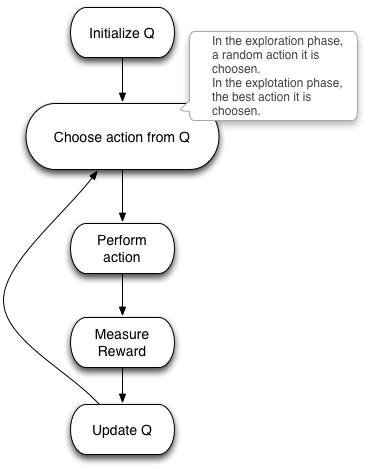
\includegraphics{./images/qalgo.png}
\caption{Q Learning algorithm}
\label{fig:qalgo}
\end{figure}


\begin{figure}[h]
\begin{minipage}{.5\textwidth}
\centering
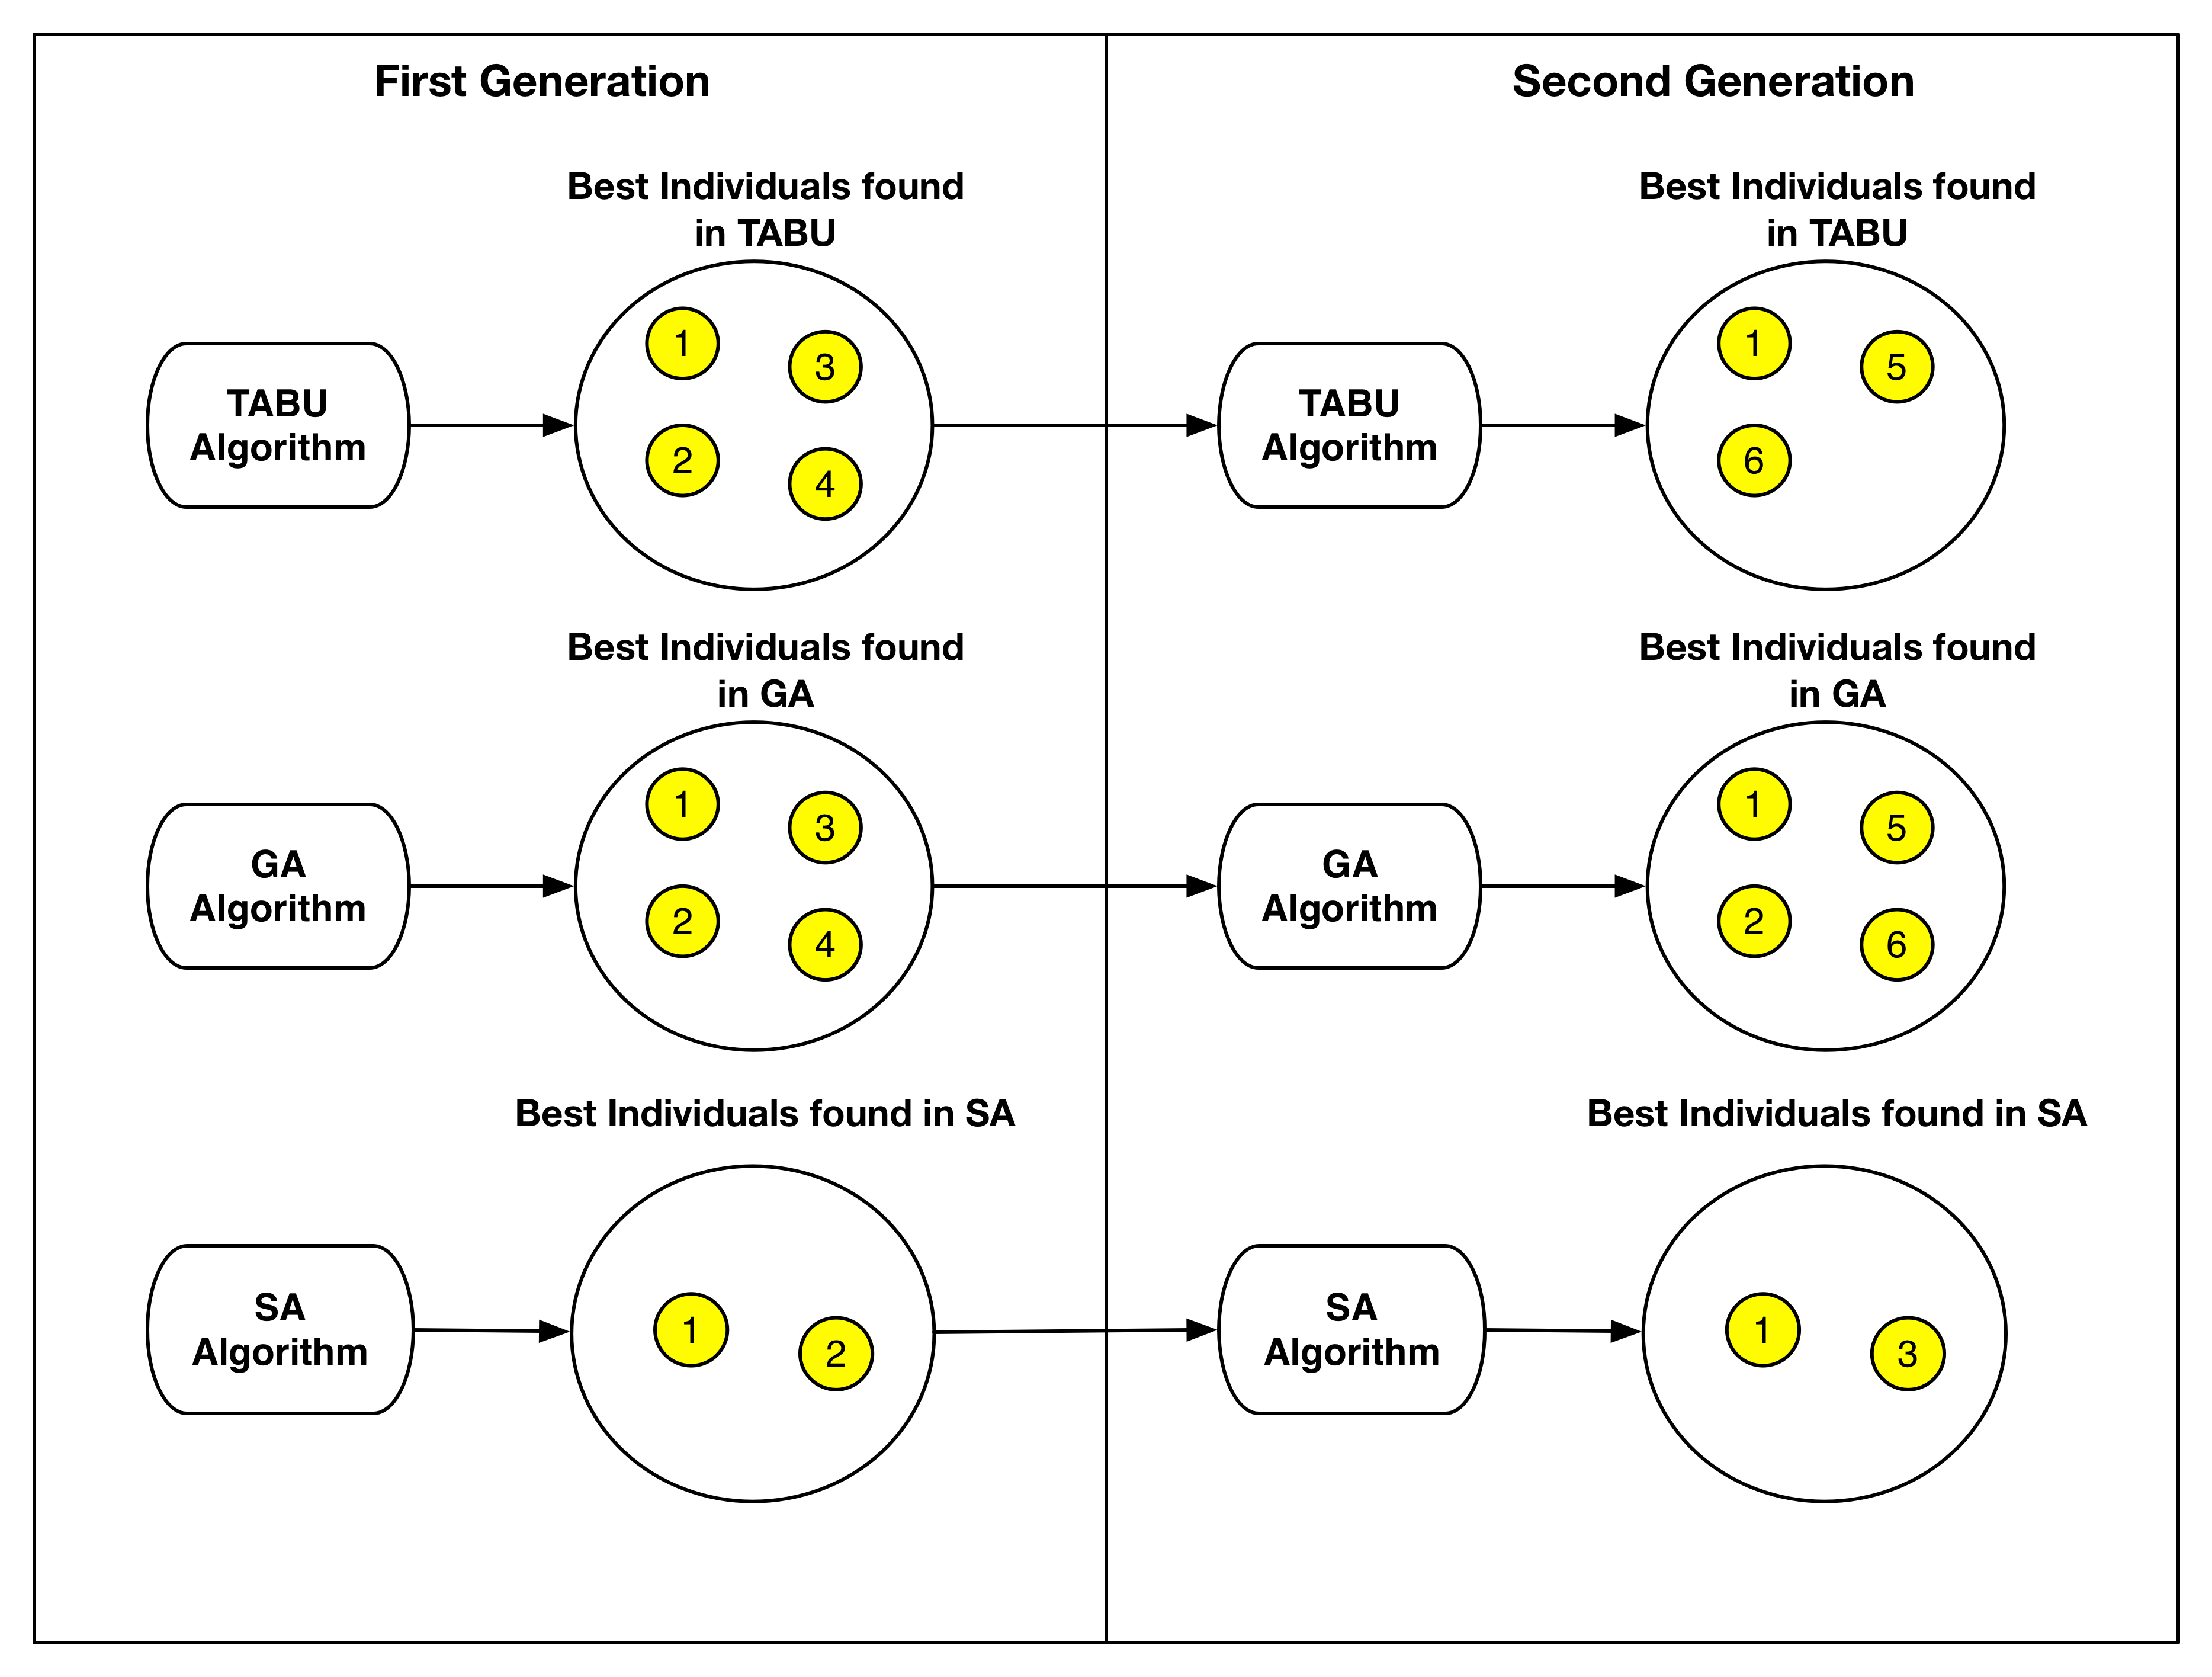
\includegraphics{./images/independ.png}
\caption{Use of the algorithms independently \citep{Gois2016}}
\label{fig:firstaproach}
\end{minipage}
\begin{minipage}{.5\textwidth}
\centering
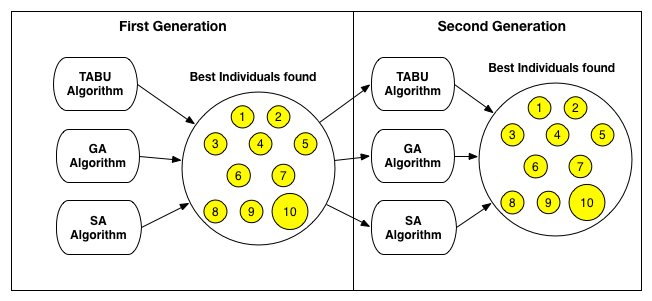
\includegraphics{./images/collaborative.png}
\caption{Use of the  algorithms collaboratively \citep{Gois2016}}
\label{fig:secondapproach}
\end{minipage}
\end{figure}


\begin{figure}[h]
\centering
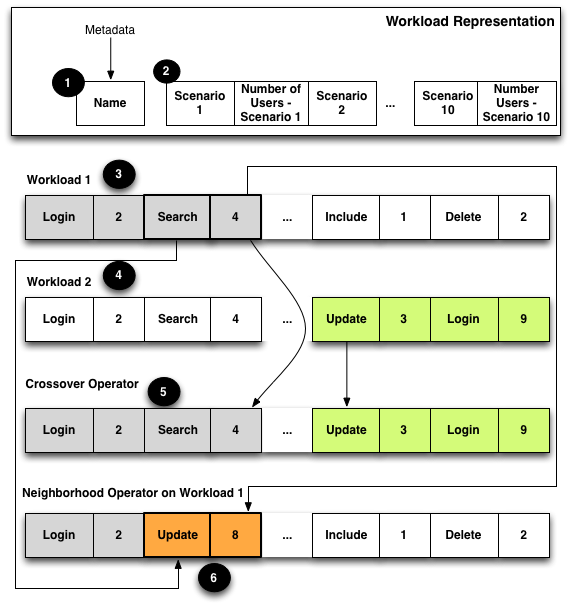
\includegraphics{./images/genomere.png}
\caption{Solution representation, crossover  and neighborhood operators \citep{Gois2016}}
\label{fig:solution}
\end{figure}

\begin{figure}[h!]
\begin{minipage}{.5\textwidth}
\center
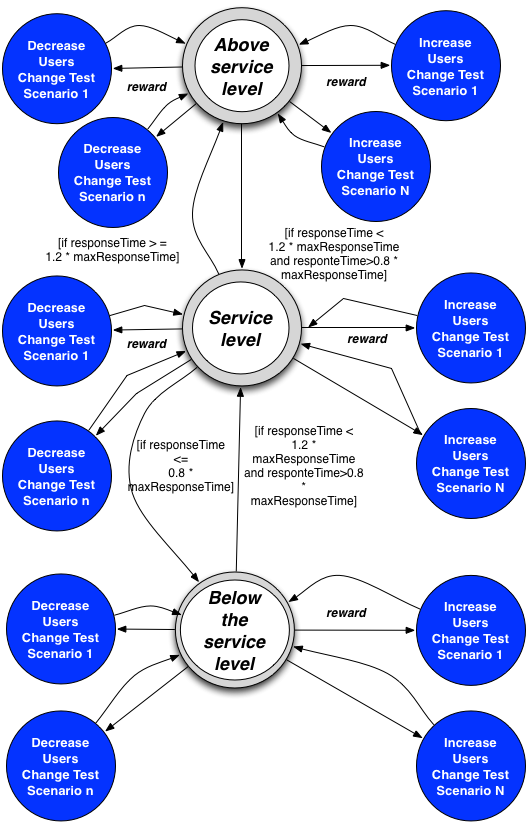
\includegraphics{./images/mdp3.png}
\caption{Markov Decision Process used by HybridQ}
\label{fig:mdphybridq}
\end{minipage}
\begin{minipage}{.5\textwidth}
\center
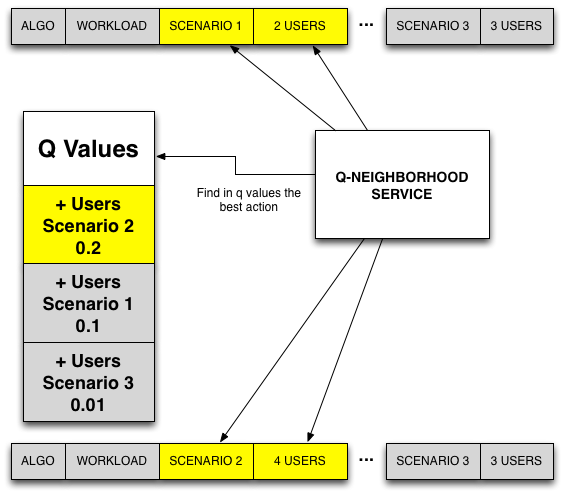
\includegraphics{./images/q-neighborservice.png}
\caption{HybridQ NeighborHood Service}
\label{fig:neighservice}
\end{minipage}
\end{figure}

\begin{figure}[h]
\centering
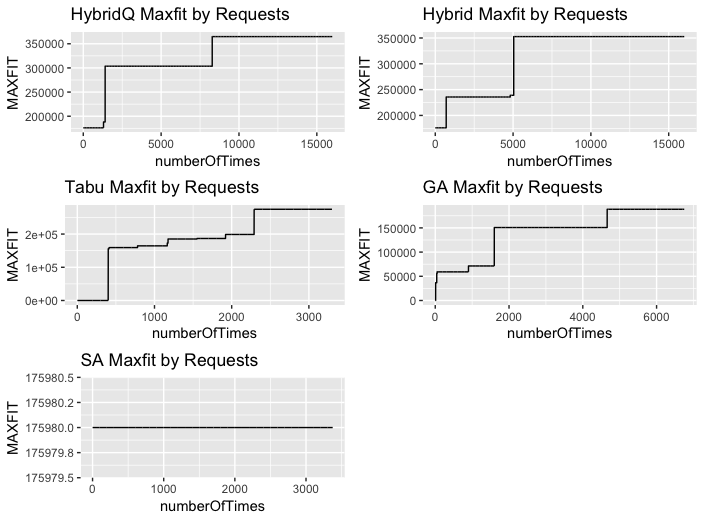
\includegraphics{./images/experiment1.png}
\caption{Maximum fitness value by number of requests}
\label{fig:experiment1}
\end{figure}




\end{backmatter}
\end{document}
